\section{Background and Related Work}
\label{sec:background}

Arguing about the security of an application running on an mainstream computer
using the x86 platform requires understanding the interactions between
all the parts of an x86 execution environment (protection modes, address
translation hardware, caches). This section provides an overview of these
features from the context of Intel TXT and SGX, touches on existing attacks on
TXT that took advantage of unexpected interactions between the features, and
points out holes in the SGX design that can be used to snoop on a program's
memory access patterns, which can reveal information about the private data
that the program is working on.


\subsection{Software Privilege Levels}
\label{sec:rings}

In an Infrastructure-as-a-Service (IaaS) cloud environment, such as Amazon EC2,
commodity CPUs run software at four different privilege levels: System
Management Mode (SMM), VMX root mode (also described as ring -1), kernel mode
(ring 0) and user mode (ring 3), as shown in Figure \ref{fig:cpu_rings}. This
section outlines the consequences of a successfully exploited vulnerability at
each privilege level, and sets the stage for analyzing the SGX protection
model.

\begin{figure}[hbtp]
  \center{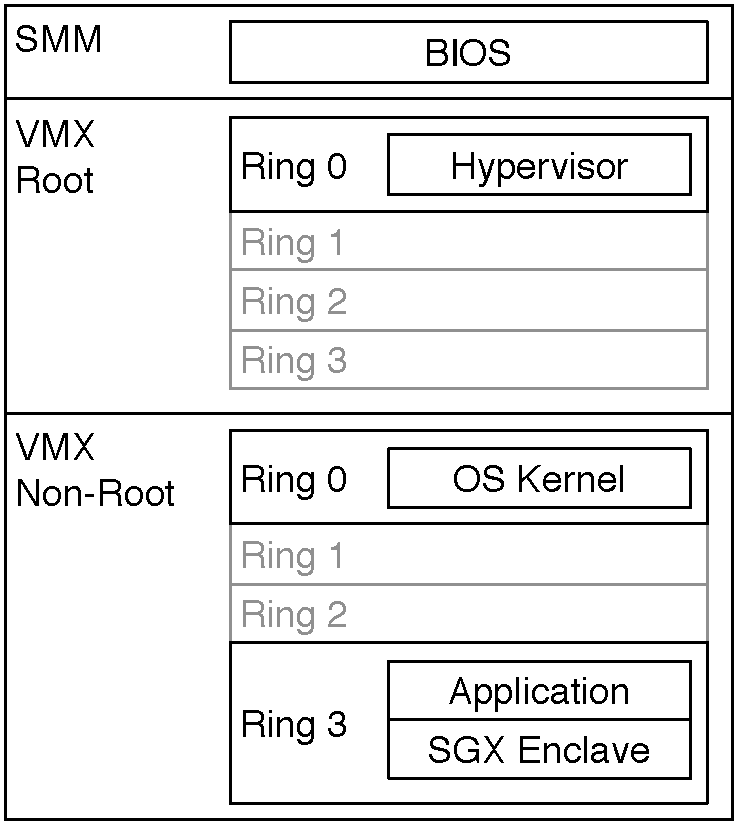
\includegraphics[width=50mm]{figures/cpu_rings.pdf}}
  \caption{
    The privilege leves in the x86 architecture, and the software that
    typically runs at each security level.
  }
  \label{fig:cpu_rings}
\end{figure}

SMM is intended for use by the motherboard manufacturers to implement features
such as fan control and deep sleep, and/or to emulate missing hardware. SMM
mode is entered by asserting the SMI\# pin on the CPU, which was initially
designed exclusively for hardware use. However, the southbridges on most
motherboards provide a method for the hypervisor and kernel to get the SMI\#
pin asserted\footnote{Most southbridges assert SMI\# when a byte is written to
port 0xb2 via the \textsc{out} opcode}. The SMM code and data are stored in a
memory area called SMRAM, which, in theory, is not readable or writable when
the processor isn't running in SMM, but its protection mechanisms were bypassed
multiple times \cite{duflot2006smm} \cite{rutkowska2008remap}
\cite{wojtczuk2009smm}, and SMM-based rootkits have been demonstrated
\cite{wecherowski2009smm} \cite{embleton2010smm}.

IaaS cloud providers allow their customers to run their operating system of
choice in a virtualized environment. Hardware virtualization
\cite{uhlig2005intel}, called Virtual Machine Extensions (VMX) by Intel,
adds support for a \textit{hypervisor} (also called a Virtual Machine Monitor
/ VMM in the Intel documentation) that runs at a higher privilege level
(VMX root mode) than OS kernels, and is responsible for allocating hardware
resources across multiple operating systems that share the same physical
machine. Hypervisor code generally runs at ring 0 in VMX root mode.

The popular Xen hypervisor uses VMX root mode for improved peformance and a
smaller codebase \cite{zhang2008xen}. \cite{mccune2010trustvisor} proposes
using a hypervisor together with Intel TXT's dynamic root of trust for
measurement (DRTM) to implement trusted execution.
\cite{vasudevan2010requirements} argues that a dynamic root of trust mechanism,
like Intel TXT, is necessary to ensure a hypervisor's integrity. Unfortunately,
any SMM attack can be used to compromise Intel TXT \cite{wojtczuk2009txt}, and
the TXT implementation is complex enough that security vulnerabilities have
been found \cite{wojtczuk2009txt2} \cite{wojtczuk2011txt}.

Mainstream operating systems have monolithic kernels that include device
drivers, filesystem code, networking stacks, and video rendering functionality,
and run at ring 0 (kernel mode). Application code, such as a Web server or
a game client, runs at ring 3 (user mode). Software running inside an SGX
enclave (isolated environment) also executes at ring 3. The OS kernel, running
at ring 0, is responsible for scheduling the execution of code inside enclaves
and for allocating hardware resources (such as RAM) to the enclaves. In IaaS
cloud environments, the virtual machine images provided by customers run in VMX
non-root mode, so the kernel runs in VMX non-root ring 0, and the application
code runs in VMX non-root ring 3. SGX is compatible with VMX, and the
hypervisor is responsible for virtualizing a processor's SGX capabilities.

The monolithic kernel design leads to many opportunities for security
vulnerabilities in kernel code. For example the Linux kernel has had a
significant number of vulnerabilities patched every year, for the past 10 years
\cite{cvedetails2014linux} \cite{chen2011linux}. Also, a successful attack on
SMM or the hypervisor trivially translates into a compromised kernel. SGX
accounts for the possibility of a compromised kernel or hypervisor with an
attestation mechanism covering an enclave's contents, and with a hardware
isolation mechanism for the software inside the enclave. In \S \ref{sec:sgx},
we argue that SGX, as it is currently documented in \cite{intel2013sgxmanual},
appears to provide integrity for the software inside the enclave, but
definitely does not provide privacy, as a compromised SMM, hypervisor, or OS
kernel can obtain the enclave's memory access patterns at high granularity.


\subsection{Address Translation}
\label{sec:paging}

Recent commodity CPUs have many address translation modes, in order to run
legacy software dating back to 1990 natively. This section only addresses the
modes used in modern 64-bit operating systems and 64-bit cloud environments.
\cite{jacob1998virtual} describes the generic concepts and applications of
address translation.

64-bit desktop operating systems use the addressing mode called IA-32e in
Intel programming manual \cite{intel2013manual}, which translates 48-bit
\textit{virtual addresses} into \textit{physical addresses} of at most 52
bits\footnote{The size of a physical address is CPU-dependent, and is 40 bits
for recent desktop CPUs and 44 bits for recent high-end server CPUs.}. Figure
\ref{fig:os_paging} illustrates the address translation process. The bottom 12
bits of a virtual address are not changed by the translation. The top 36 bits
are grouped into four 9-bit indexes used to navigate a data structure called
\textit{the page tables}. Despite its name, the data structure closely
resembles a perfectly balanced 512-ary search tree where the nodes do not store
keys. Each node is an array of 512 8-byte entries that contain the physical
addresses of the next-level children as well as some flags. The address of the
root node is stored in the CR3 register. The arrays in the last-level nodes
contain the physical addresses that are the result of the address translation.

\begin{figure}[hbtp]
  \center{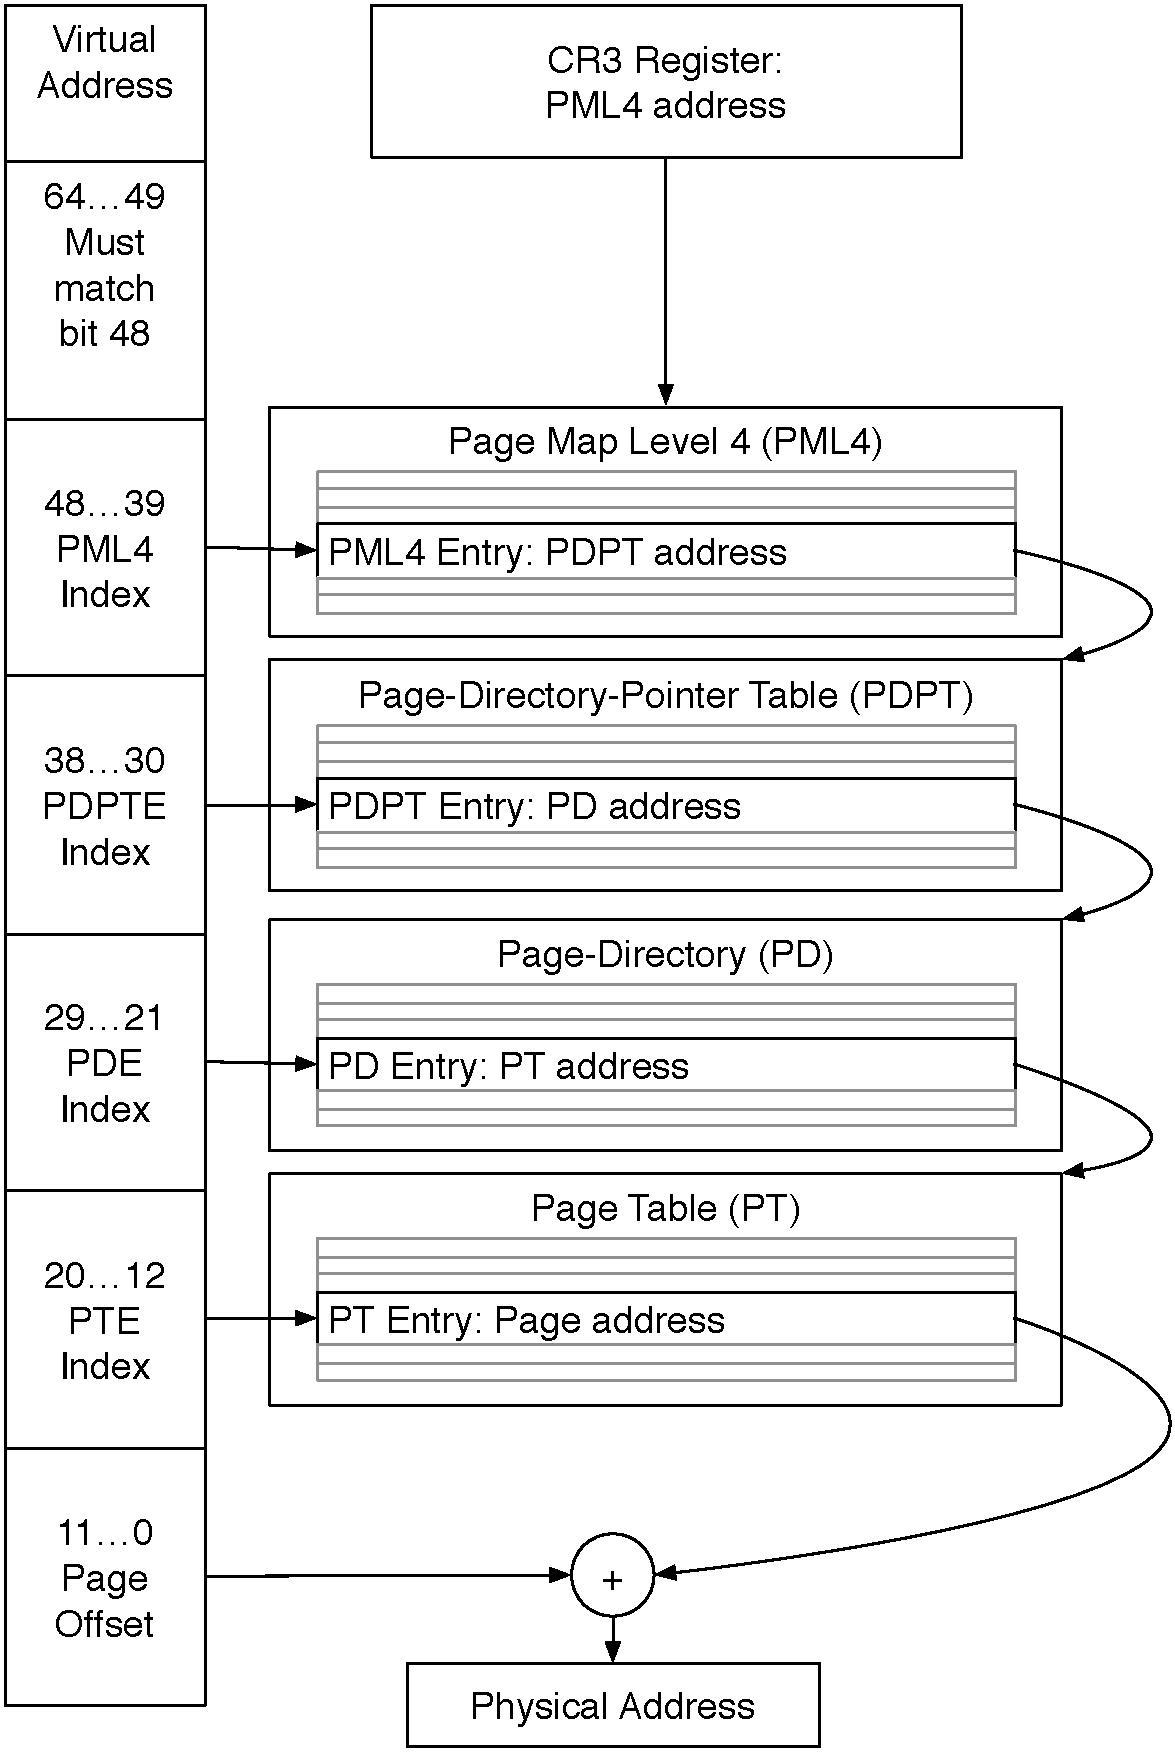
\includegraphics[width=85mm]{figures/os_paging.pdf}}
  \caption{
    IA-32e address translation takes in a 48-bit virtual address and outputs
    a 52-bit physical address.
  }
  \label{fig:os_paging}
\end{figure}

Hardware virtualization (used in cloud computing) allows a hypervisor to run
multiple operating systems concurrently using the same physical memory, by
adding another layer of address translation. When extended page tables (EPT)
are enabled, the process above is used to translate from a virtual address into
a \textit{guest-physical address}. The translation from guest-physical
addresses to actual physical addresses uses the same process as above, except
the physical address of the root node is stored in the extended page table
pointer (EPTP) field in the VM's control structure (VMCS). Figure
\ref{fig:vmx_paging} illustrates the address translation process in the
presence of hardware virtualization.

\begin{figure}[hbtp]
  \center{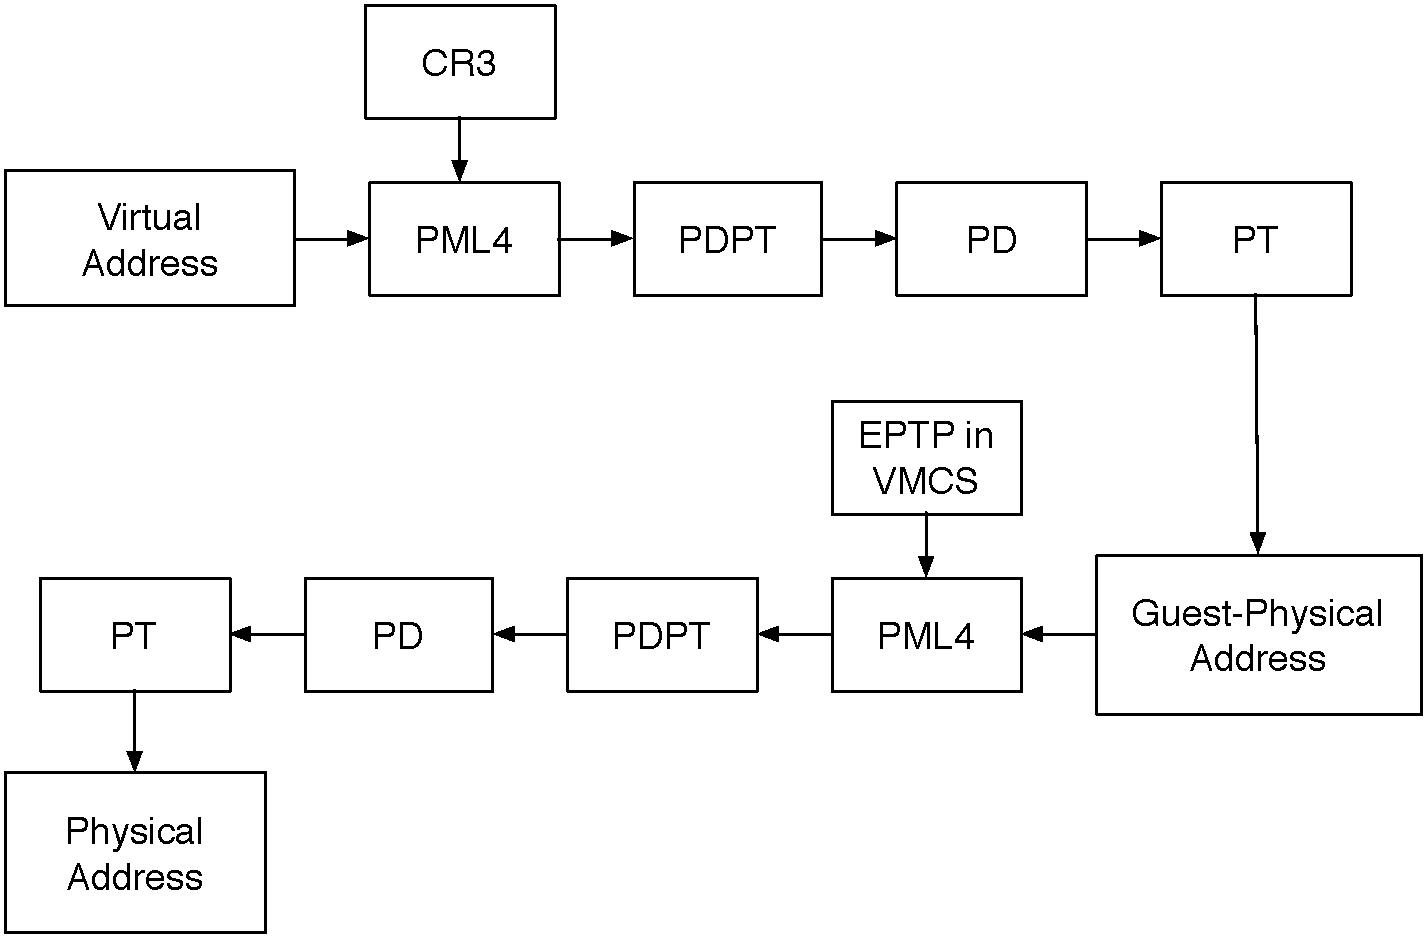
\includegraphics[width=85mm]{figures/vmx_paging.pdf}}
  \caption{
    Address translation when hardware virtualization is enabled. A translation
    requires up to 8 memory accesses.
  }
  \label{fig:vmx_paging}
\end{figure}

Each entry in the page tables has some boolean flags, in addition to the
pointer to the next level. The following flags are particularly interesting for
our goals. The \textit{present} (P) flag is set to 0 to indicate pages that
have been evicted from RAM to a cheaper and slower storage medium. When address
translation encounters a page table entry where P is 0, the CPU generates a
page fault (\#PF), and the OS kernel is responsible for loading the page back
into RAM and resuming execution. If an extended page table (EPT) entry has the
P flag set 0, the CPU performs a VM exit, and the hypervisor has an opportunity
to bring the page into RAM. The \textit{accessed} (A) flag is set to 1 by the
CPU whenever the address translation machinery reads a page table entry, and
the \textit{dirty} (D) flag is set to 1 by the CPU when an entry is accessed by
a memory write operation. The A and D flags give the hypervisor and OS kernel
insight into application memory access patterns, providing the input for the
algorithms that select which pages get be evicted from RAM.

Page table entries have flags that provide access control, in addition to the
flags supporting page swapping. The interesting flags are the \textit{writable}
(W) flag, which can be set to 0 to prohibit\footnote{Writes to non-writable
pages result in general protection faults (\#GP).} memory writes to a page, and
the \textit{disable execution} (XD) flag, which can be set to 0 to prevent
instruction fetches from a page.

Address translation applies to the software running in an SGX enclave
(isolated environment). This means that both the OS kernel and the hypervisor
have an impact over the mapping of virtual addresses to physical addresses, and
either of them can take advantage of the features above to obtain the SGX
application's memory access pattern, at page granularity, as detailed in
\S \ref{sec:sgx_leaks}.


\subsection{CPU Caches}
\label{sec:caching}

Desktop-class multi-core commodity CPUs have three levels of cache memory. Each
core has its own L1 and L2, and all cores share an L3 cache. All cache levels
are located on the CPU die so, according to our threat model, they can be
trusted. In particular, we can assume that software memory reads and writes for
locations that are already cached (and therefore do not generate DRAM requests)
cannot be directly observed by an attacker. This requires that the software's
memory is confirmed to be cacheable with a write-back policy, and our system
accounts for this requirement.

Cache accesses can be indirectly observed by various timing attacks
\cite{banescu2011cache}, by malicious software that time-shares a CPU or a core
with the targeted software and takes advantage of a specific cache's layout
and replacement algorithms. Our system prevents against these attacks, also by
taking advantage of some details of the cache implementation on commodity CPU
processors. This section describes the aspects that we rely on.
\cite{smith1982cache}, \cite{patterson2013architecture} and
\cite{hennessy2012architecture} all provide good backgrounds on low-level cache
implementation concepts.

The \textit{cache line} is the atomic unit of data transfer between the caches
and the main memory. The cache line size is always a power of two. Assuming
$n$-bit memory addresses and a cache line size of $2^{l}$ bytes, the lowest
$l$ bits of a memory address are an offset into a cache line, and the highest
$n - l$ bits determine the cache line that is used to store the data at the
memory location. All recent processors have 64-byte cache lines.

The L1 and L2 caches in recent processors are multi-way set-associative with
direct set indexing, as shown in Figure \ref{fig:cpu_cache}. An $W$-way
set-associative cache has its memory divided into \textit{sets}, where each set
has $W$ lines. A memory location can be cached in any of the $w$ lines in a
specific set that is determined by the highest $n - l$ bits of the location's
memory address. Direct set indexing means that the $S$ sets in a cache are
indexed from $0$ to $S - 1$, and a memory location is cached in the set with
index $address_{n - 1 \ldots n - l} \bmod S$. In the common case where the
number of sets in a cache is a power of two, so $S = 2^{s}$, the lowest $l$
bits in an address make up the cache line offset, the next $s$ bits are the set
index. The highest $n - s - l$ bits in an address are not used when selecting
where a memory location will be cached. Figure \ref{fig:cpu_cache} shows the
cache structure and lookup process.

\begin{figure}[hbtp]
  \center{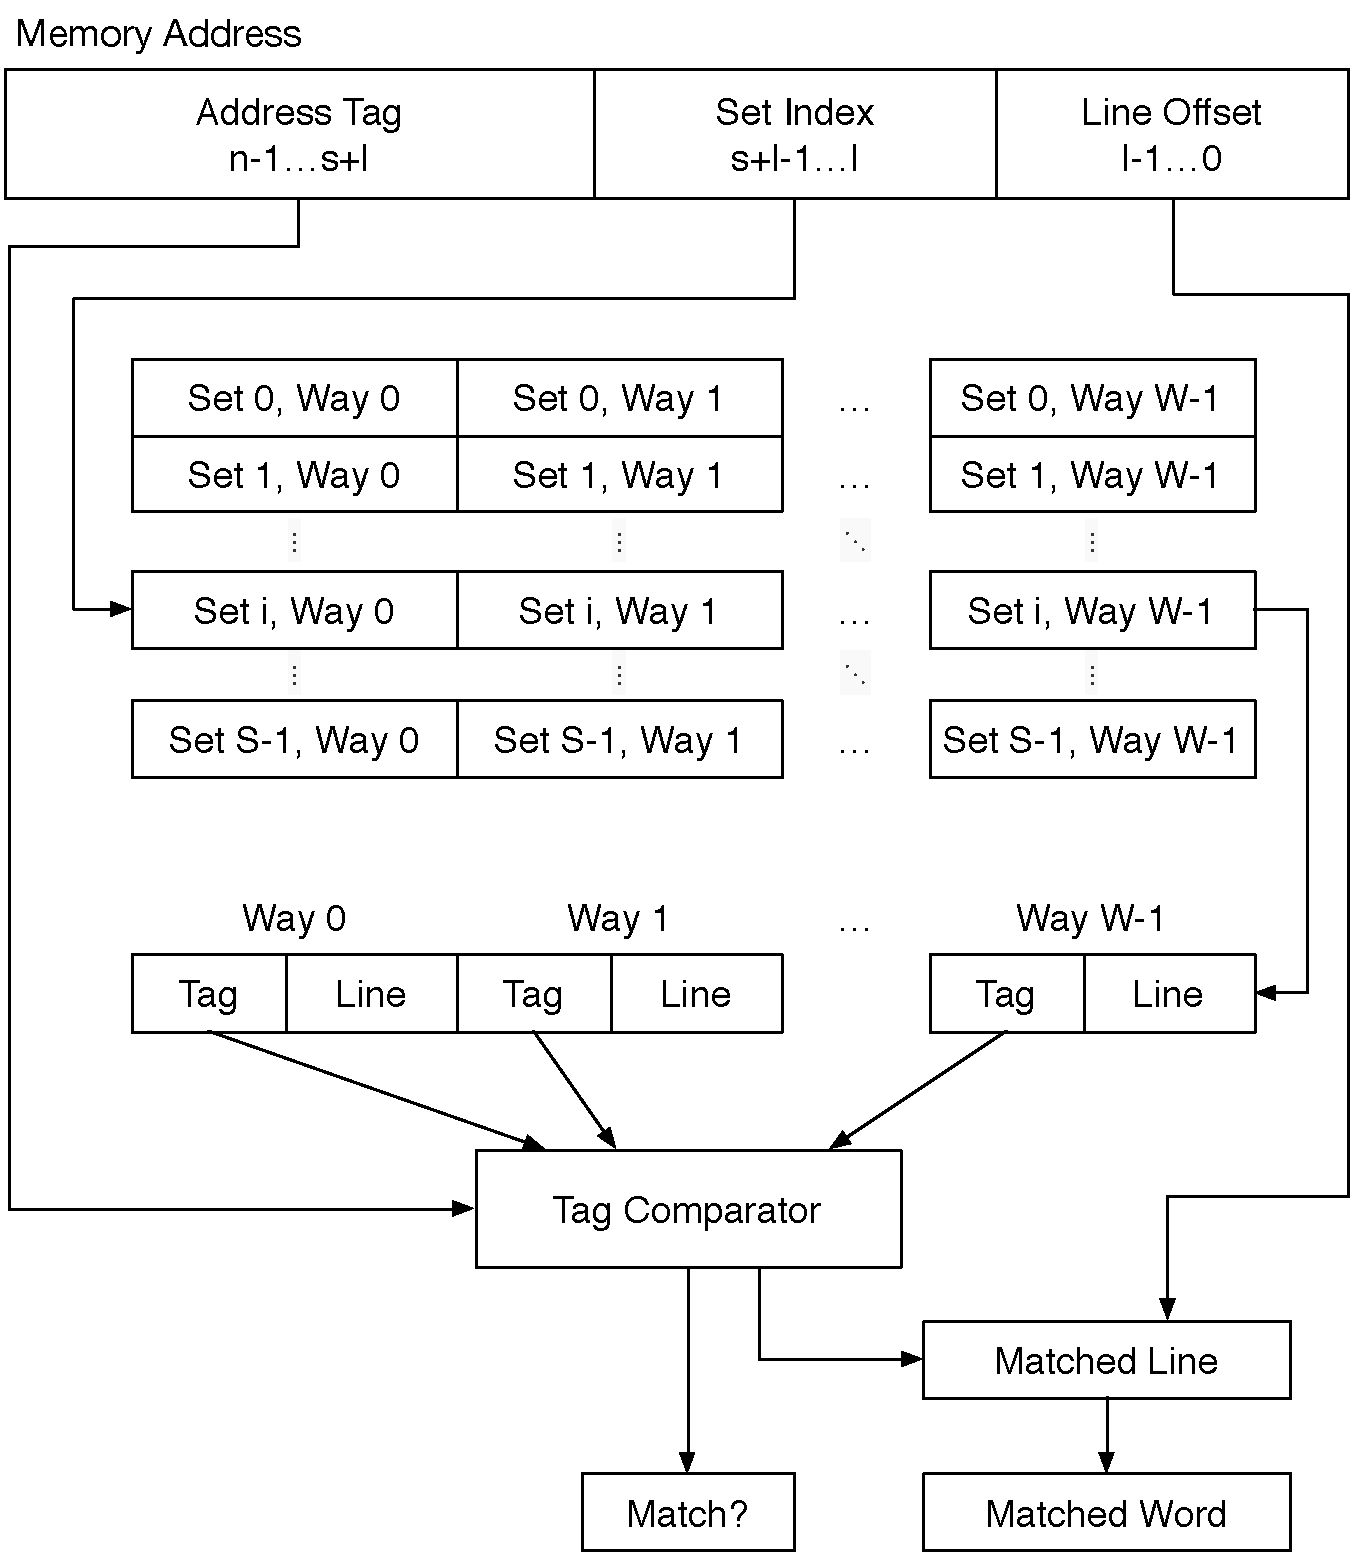
\includegraphics[width=85mm]{figures/cpu_cache.pdf}}
  \caption{
    Cache organization and lookup, for a $W$-way set-associative cache with
    $2^{l}$-byte lines and $S = 2^{s}$ sets. The cache works with $n$-bit
    memory addresses. The lowest $l$ address bits point to a specific byte in a
    cache line, the next $s$ bytes index the set, and the highest $n - s - l$
    bits are used to decide if the desired address is in one of the $W$ lines
    in the indexed set.
  }
  \label{fig:cpu_cache}
\end{figure}

According to the CPUID instruction results and the Intel programming manuals
\cite{intel2013manual}, the L3 cache of recent processors does not use direct
set indexing, and instead uses a ``complex'' indexing scheme. The manuals do
not describe the scheme, so our system cannot rely on the L3 cache. Due to the
lack of a specification, our system must treat the L3 cache as untrusted
memory. This is rather unfortunate because, although the shared aspect of the
L3 cache would introduce additional complexity in a design, its large size
(30MB on high-end CPUs, compared to 256KB of per-core L2 cache) would make
``taming'' this last level of cache memory very attractive.

\subsection{Caching and Address Translation}

Address translation (described in \S \ref{sec:paging}) requires 4 memory
accesses for a 64-bit bare-metal kernel, and 8 memory accesses when a
hypervisor is present. To achieve high clock speeds, the CPU caches address
translations in a TLB (translation look-aside buffer). The set index in an L1
cache only uses the address bits that are not impacted by address translation,
so that set lookup and TLB lookup can be done in parallel. Given a page size
$P = 2^{p}$ bytes, the requirement above is equivalent to $l + s \le p$. In the
x86 architecture $p = 12$, and all recent processors have 64-byte cache lines
($l = 6$) and 64 sets ($s = 6$), as shown in Figure
\ref{fig:caching_and_paging}.

\begin{figure}[hbtp]
  \center{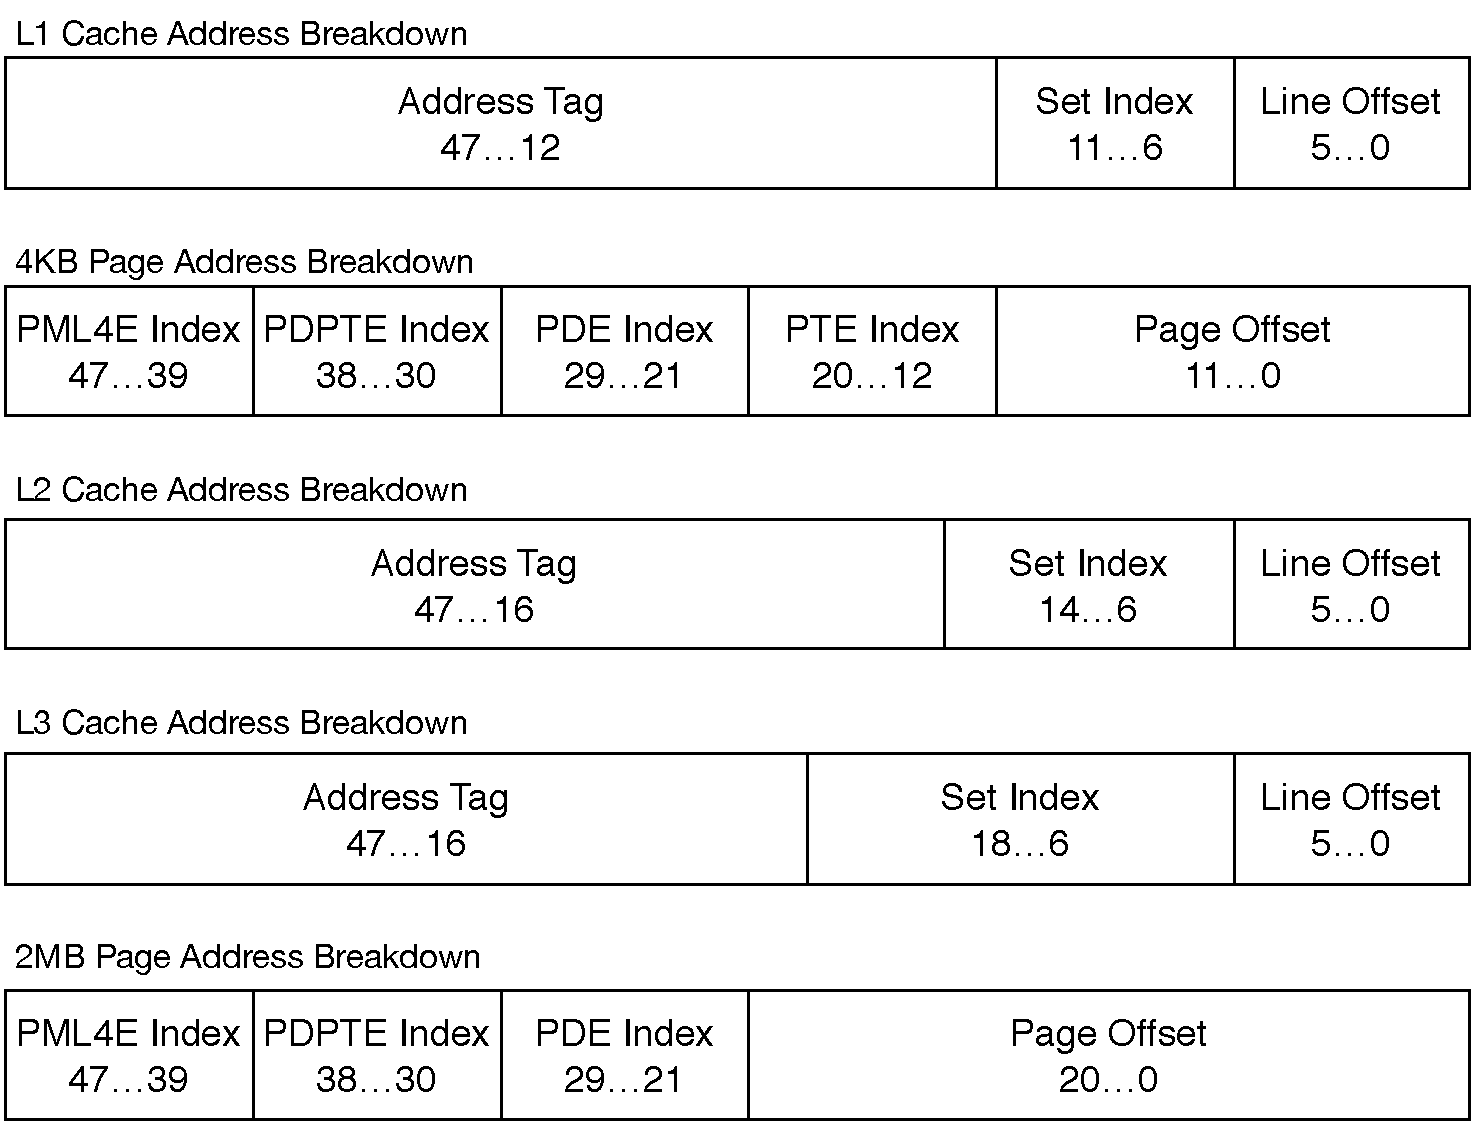
\includegraphics[width=85mm]{figures/caching_and_paging.pdf}}
  \caption{
    Virtual addresses from the perspective of cache lookup and address
    translation. The bits used for the L1 set index and line offset are not
    changed by address translation, so the page tables do not impact L1 cache
    placement. Page tables do impact L2 and L3 cache placement. Using large
    pages (2MB or 1GB) makes cache placement independent of page tables.
  }
  \label{fig:caching_and_paging}
\end{figure}

The L2 cache in recent Intel processors uses physical indexing
\cite{patterson2013architecture}. The indexing method is not documented in
Intel's manuals and is not reported by the CPUID instruction, as it is
considered to be an implementation detail. However, the indexing method
determines the set index for a given memory location, and knowing which memory
addresses are stored in the same set is crucial for mounting and defending
against cache timing attacks.
